\chapter{肌肉结构和动力学} \label{chap:chap5}


如果你想理解功能,那就研究结构。

\begin{flushright}
	——弗朗西斯$\cdot$克里克
\end{flushright}


\begin{figure}[!htb]
	\centering
	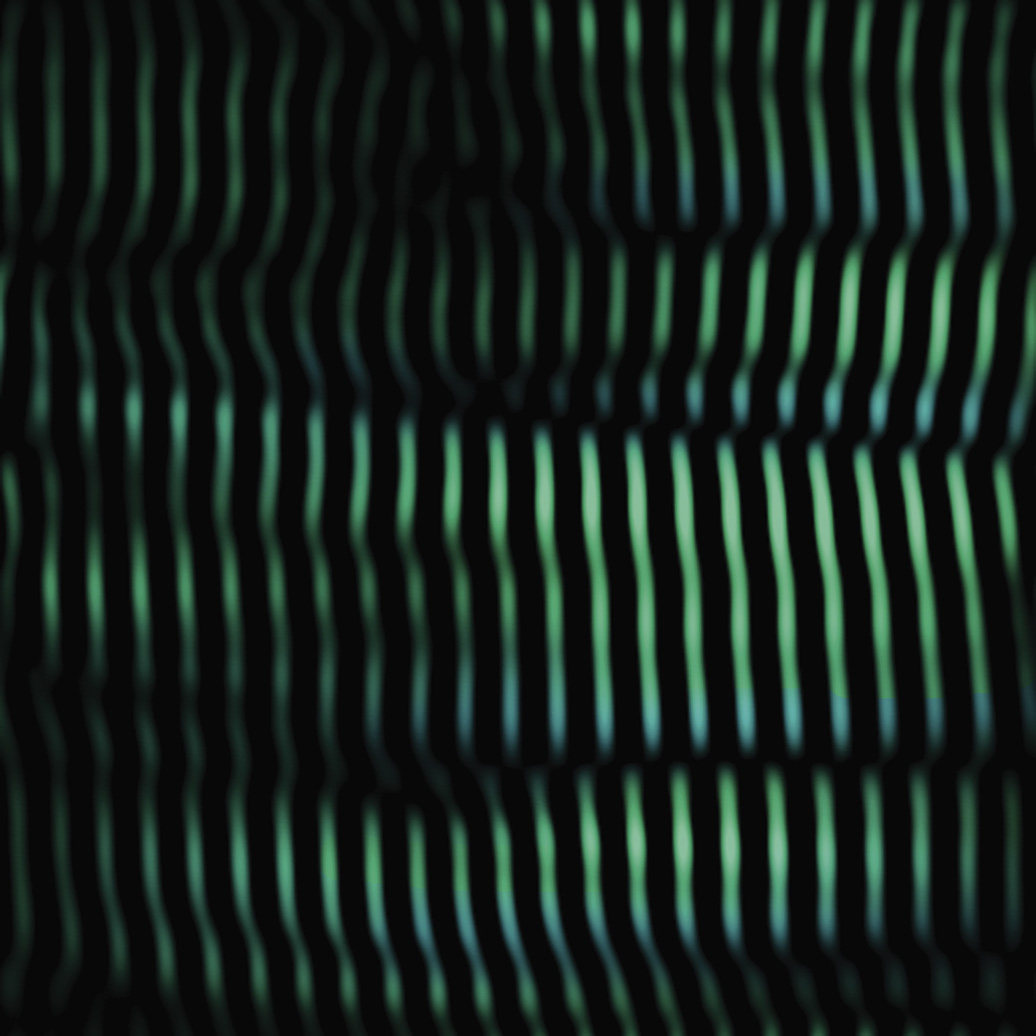
\includegraphics[width=1.0\linewidth]{chap4/4_0}
	% 加星号(*)表示不加编号
	\caption*{ \label{fig:5_0}}
\end{figure}


为了理解人类和动物的运动,研究人员开展了各种各样的实验。
生物力学家通过测量数千人的关节运动、地面反作用力和肌电信号来研究全身运动。
生理学家研究了单个肌肉,以表征肌肉激活和力量产生的动态。
肌肉驱动模拟使我们能够将这两个领域联系起来,将全身运动的生物力学测量与针对单个肌肉进行的实验相结合。
我们将在第~\ref{chap:chap10}~至~\ref{chap:chap12}~章中看到,肌肉驱动模拟可以深入了解肌肉在产生运动中的作用,并提供一些在人体运动时几乎无法测量的重要量的估计值,例如肌肉产生的力量和它消耗的能量。


肌肉动力学建模对于创建肌肉驱动的运动模拟至关重要。
然而,一刀切的模型并不适用,因为每块肌肉都有其独特的结构来适应其独特的功能。
例如,一些肌肉负责手指的精细运动控制,而另一些肌肉则在运动过程中支撑身体重量(图~\ref{fig:5_1})。
所有骨骼肌都具有肌节的层级排列,但肌肉在几个重要方面存在差异。
这些差异包括它们的大小和结构,以及肌肉纤维的几何排列。
因此,肌肉的计算模型必须捕捉所有肌肉共同的肌肉力量产生特征,同时还要能够表征每块肌肉的独特特征。


\begin{figure}[!htb]
	\centering
	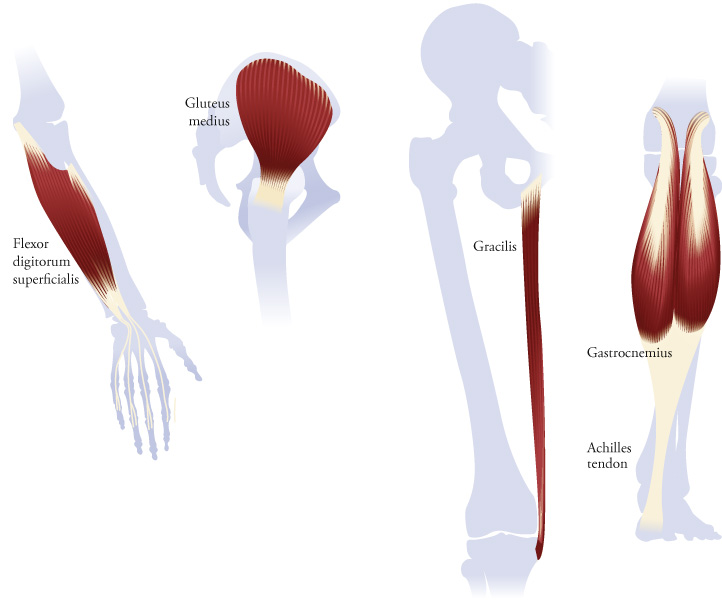
\includegraphics[width=1.0\linewidth]{chap5/5_1}
	\caption{全身肌肉的结构和功能各不相同。
		浅屈指肌(最左侧)通过四条肌腱控制手指屈曲;
		宽阔的臀中肌和纤细的股薄肌产生髋关节外展和内收力矩;
		腓肠肌(最右侧)通过较长的跟腱止于跟骨。 \label{fig:5_1}}
\end{figure}


在本章中,我们将了解如何创建一个通用的肌肉力量产生模型,以及如何对其进行定制以代表身体中的几乎任何肌肉。
我们将要描述的肌肉模型属于以 A. V. Hill 命名的一类模型,除了我们在第~\ref{chap:chap4}~章中看到的“推我拉你”实验之外,他还进行了许多肌肉的基础研究。
我的博士生导师 Felix Zajac 改进了 Hill 型模型,并将其带入了现代计算机模拟时代\cite{zajac1989muscle}。
具体来说,Zajac 开发了一个仅包含四条通用曲线和五个肌肉特定参数的模型,所有这些参数都可以从实验数据中得出并用于调整模型。
Zajac 模型的简单性对于涉及数十块肌肉的动态模拟至关重要,但它足够详细,可以表示不同大小、强度和结构的肌肉的动态。


图~\ref{fig:4_18}~总结了所有肌肉共同的肌肉力量产生特征。
这些特征包括 3 条曲线,描述肌肉长度与其产生的力之间的非线性关系:主动力-长度曲线、被动力-长度曲线和力-速度曲线。
由于肌肉通过肌腱附着在骨骼上,我们还必须考虑这种结缔组织的特性,我们用肌腱的力-长度曲线来描述它。
我们使用 5 个参数缩放这些通用曲线以表示特定的肌肉:
(1)最佳肌纤维长度 $l_o^M$;
(2)最佳纤维长度下的肌纤维羽状角 $\phi_o$ ;
(3)最大等长肌肉力量,$F_o^M$;
(4)最大肌肉收缩速度 $v_\text{max}^M$;
和(5)肌腱松弛长度,$l_s^T$。
本章首先介绍这 5 个特定于肌肉的参数。
我们将了解每个参数如何影响肌肉力量,并将其纳入肌肉-肌腱动力学模型中。


